
\begin{figure}
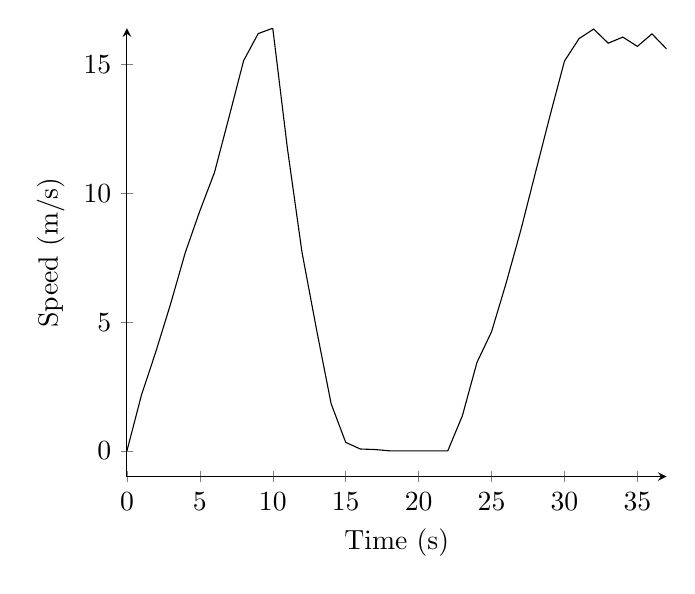
\begin{tikzpicture}
\begin{axis}[
legend style={anchor=west},
axis x line=bottom,
axis y line=left,
ymin=-1,
xlabel=Time (s),
ylabel=Speed (m/s),
]
\addplot[] coordinates {
(0, 0.0)
(1, 2.17125535361)
(2, 3.88159123773)
(3, 5.71844061662)
(4, 7.69993032853)
(5, 9.32092533156)
(6, 10.8076631732)
(7, 12.9626629478)
(8, 15.1560121533)
(9, 16.2094614887)
(10, 16.4174697059)
(11, 11.7635403415)
(12, 7.72548094203)
(13, 4.71082722229)
(14, 1.83020507534)
(15, 0.327779109853)
(16, 0.0705589072029)
(17, 0.0493178492736)
(18, 0.0)
(19, 0.0)
(20, 0.0)
(21, 0.0)
(22, 0.0)
(23, 1.36234863628)
(24, 3.43446519184)
(25, 4.62565311684)
(26, 6.517522245)
(27, 8.55818695056)
(28, 10.7859800598)
(29, 13.0006347593)
(30, 15.1413450439)
(31, 16.0146006578)
(32, 16.3850160371)
(33, 15.835987959)
(34, 16.0725623151)
(35, 15.7118808856)
(36, 16.1982950972)
(37, 15.6118437874)
};

\end{axis}
\end{tikzpicture}
\label{tik:0:12_O, 13_S, 14_O}
\caption{0 percent diving with GSC on route $12_O, 13_S, 14_O$}
\end{figure}
